\section{Geometría y Ciclo Operativo del MRCVC}
%
Un análisis de la geometría y la duración del ciclo del MRCVC se realizó en
trabajos anteriores~\parencite{mrcvc_geom}, en este apartado se destacaran
algunos de los aspectos geométricos del motor.
%
Los componentes principales del motor son: rotor, estator, paletas y bieletas,
rueda paralelizadoras, eje de motor, conducto de admisión y conducto de escape;
el motor analizado en este trabajo tiene 3 paletas con ápices agudos, que
corresponden a la geometría ideal del motor (sin sellos).
%
La forma de estos elementos se puede ver en la figura~\ref{fig:mrcvc} y en la
tabla~\ref{tab:geom_mrcvc} donde se resumen los parámetros geométricos que
corresponden al motor analizado en este trabajo y anteriores.

% Para un motor de $n$ paletas de radio de punta nulo, la geometría como función
% del ángulo del cigüeñal queda totalmente definida por el radio de trayectoria
% de paletas $R$, semi ancho de paletas $r$ y altura de cámara $h$.

Uno de los aspectos más importantes de este motor es que la geometría de la
cámara de combustión es tal que el volumen mínimo del ciclo permanece constante
por un período angular definido por la geometría del motor. 
%
Este período es lo suficientemente grande para permitir que la combustión se
realice casi en su totalidad a volumen constante y ya se vio en el apartado
\ref{capitulo:2_MCI} los motivos por lo que esto es beneficioso.
%
El balanceo de fuerzas que se obtiene por ser un motor rotativo permite operar
el motor a altas RPM, permitiendo alcanzar mayores potencias que motores de 
tamaño o cilindrada similar.

Para un motor de $R=\lua{tex.print(myData.R)}$ mm y
$r=\lua{tex.print(myData.r)}$ mm  el volumen mínimo alcanzado permanece
constante por un período de $44.65^\circ$ grados, como se puede ver en la
figura~\ref{fig:vol_constante} en donde se esquematiza la variación del volumen
con respecto al ciclo.

\begin{figure}
    \centering
    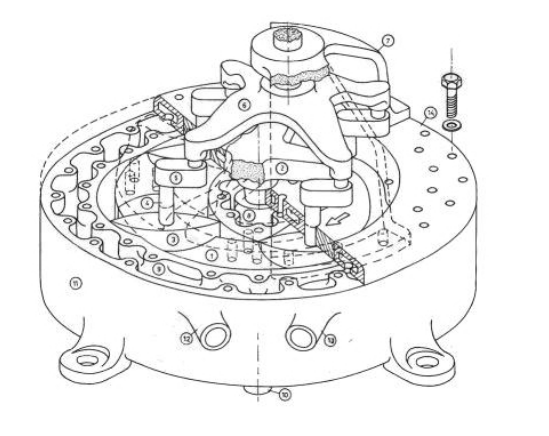
\includegraphics[width=0.7\textwidth]{perspectiva_mrcvc.png}
    \caption{MRCVC\parencite{mrcvc_geom}}\label{fig:mrcvc}
\end{figure}

\begin{figure}
    \centering
    \begin{tikzpicture}
        \begin{axis}[
            xlabel=Angulo $(deg)$,
            ylabel=Volumen $(mm^3)$,
            grid=major,
            mark size=0pt,
        ]
        \addplot table [x=Angle,y=Volume] {data/vol.dat};
        \end{axis}
    \end{tikzpicture}
    \caption{Variación del volumen del MRCVC de 3 paletas}
    \label{fig:vol_constante}
\end{figure}

\begin{table}
    \centering
    \begin{tabular}{rcc} \toprule
        Parámetro & Valor                            & Unidades \\ \midrule
        n         & \lua{tex.print(myData.n)}        & --- \\
        R         & \lua{tex.print(myData.R)}        & mm \\
        r         & \lua{tex.print(myData.r)}        & mm \\
        $h_c$     & \lua{tex.print(myData.hc)}       & mm \\
        rc        & \lua{tex.print(myData.rc)}       & --- \\
        V0        & \lua{tex.print(myData.V0)}       & $cm^3$ \\
        $R_i$     & \lua{tex.print(trunc(myData.Ri))} & mm \\
        $R_e$     & \lua{tex.print(trunc(myData.Re))} & mm \\ \bottomrule
    \end{tabular}
    \caption{Geometría del MRCVC}\label{tab:geom_mrcvc}
\end{table}

Los ángulos que determinan el reglaje de los puertos de admisión y escape son
los de apertura y de cierre del puerto.
%
Como ejemplo, la posición del puerto de escape queda determinada por los
valores \emph{EIA} y \emph{EFA} como se ve en la
figura~\ref{fig:angulos_escape} para el puerto de escape.

\begin{figure}
    \centering
    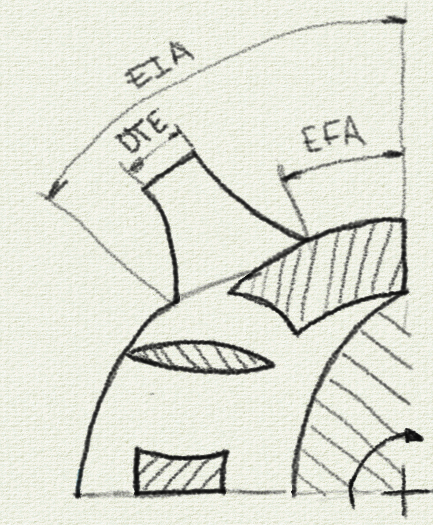
\includegraphics[width=0.5\textwidth]{angulos_escape.png}
    \caption{Puerto de escape}\label{fig:angulos_escape}
\end{figure}


% %%%%%%%%%%%%%%%%%%%%%%%%%%%%%%%%%%%%%%%%%%%%%%%%%%%%%%%%%%%%%%%%%%%%%%%%%%%%%%%
%
% \subsection{Geometría}
% %
% La geometría del MRCVC permite que gran parte de la combustión se de a volumen
% constante\parencite{mrcvc_geom}, como se puede ver en la figura~\ref{fig:vol_constante},
% en donde se esquematiza la variación del volumen con respecto al ciclo.
%
% \begin{figure}
%     \centering
%     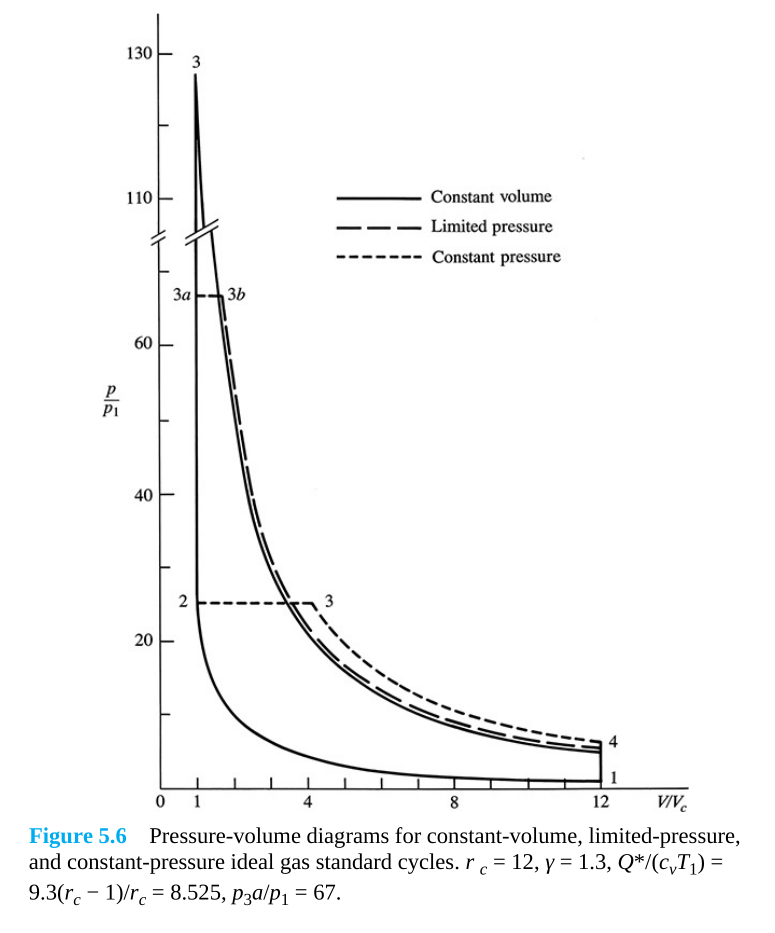
\includegraphics[width=0.7\textwidth]{comparacion_ciclos.png}
%     \caption{Comparación de ciclos ideales (cambiar por una imagen propia)}\label{fig:comparacion_ciclos}
% \end{figure}
%
%
% Para un motor de $n$ paletas de radio de punta nulo, la geometría como función
% del ángulo del cigüeñal queda totalmente definida por el radio de trayectoria de
% paletas $R$, semi ancho de paletas $r$ y altura de cámara $h$.
%
% \begin{figure}
%     \centering
%     \begin{tikzpicture}
%         \begin{axis}[
%             xlabel=Angulo $(deg)$,
%             ylabel=Volumen $(mm^3)$,
%             grid=major,
%             mark size=0pt,
%         ]
%         \addplot table [x=Angle,y=Volume] {data/vol.dat};
%         \end{axis}
%     \end{tikzpicture}
%     \caption{Combustión a volumen constante}\label{fig:vol_constante}
% \end{figure}
%
% La geometría utilizada para este trabajo se resumen en la
% tabla~\ref{tab:geom_mrcvc} y se ilustra en la figura~\ref{fig:geom_mrcvc}.
% %
% Esta geometría es la continuación de la utilizada en trabajos anteriores, con la
% cual se realizó parte del prediseño del sistema de intercambio de gases.
%
% \begin{table}
%     \centering
%     \begin{tabular}{rcc} \toprule
%         Parámetro & Valor                            & Unidades \\ \midrule
%         n         & \lua{tex.print(myData.n)}        & unidades \\
%         R         & \lua{tex.print(myData.R)}        & mm \\
%         r         & \lua{tex.print(myData.r)}        & mm \\
%         $h_c$     & \lua{tex.print(myData.hc)}       & mm \\
%         rc        & \lua{tex.print(myData.rc)}       & --- \\
%         V0        & \lua{tex.print(myData.V0)}       & $cm^3$ \\
%         $R_i$     & \lua{tex.print(trunc(myData.Ri))} & mm \\
%         $R_e$     & \lua{tex.print(trunc(myData.Re))} & mm \\
%     \end{tabular}
%     \caption{Geometría del MRCVC}\label{tab:geom_mrcvc}
% \end{table}
%
% Los ángulos que determinan el reglaje de los puertos de admisión y escape son los
% de inicio y de cierre del puerto.
% %
% Como ejemplo, la posición del puerto de escape queda determinada por los  valores
% EIA y EFA como se ve en la figura~\ref{fig:angulos_escape}.
%
% \begin{figure}
%     \centering
%     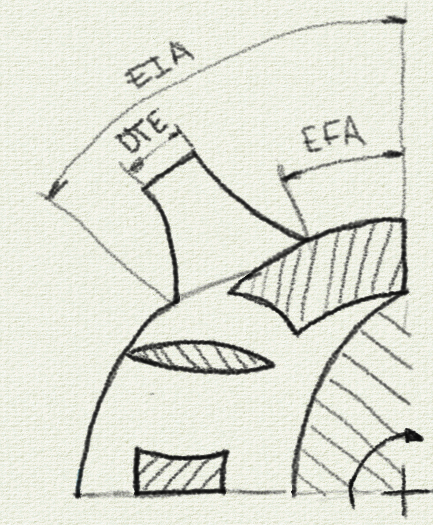
\includegraphics[width=0.5\textwidth]{angulos_escape.png}
%     \caption{Puerto de escape}\label{fig:angulos_escape}
% \end{figure}
%
% % NOTA: esto deberia ir en la parte de geometria de los puertos, luego de la
% % primer iteracion de opttimizacion
%
% % Como se puede ver en la figura~\ref{fig:primeros_puertos}, se buscó suavizar los
% % vértices en donde la pared del puerto intersecta la cámara de combustión.
%
% %%%%%%%%%%%%%%%%%%%%%%%%%%%%%%%%%%%%%%%%%%%%%%%%%%%%%%%%%%%%%%%%%%%%%%%%%%%%%%%
%
% \subsection{Ciclo operativo}
% %
% La variación de la geometría y el funcionamiento en detalle de ICESym, así como
% también el modelo de solape de cámaras desarrollado para el uso con el MRCVC.\@
% %
% Para una misma relación de compresión, una combustión a volumen constante
% alcanza valores de presión y temperatura mayores en comparación a otros ciclos.
% %
% En la figura~\ref{fig:comparacion_rendimientos} se ve como para una $r_c$ dada,
% el ciclo a volumen constante tiene el mayor rendimiento.
%
% \begin{figure}
%     \centering
%     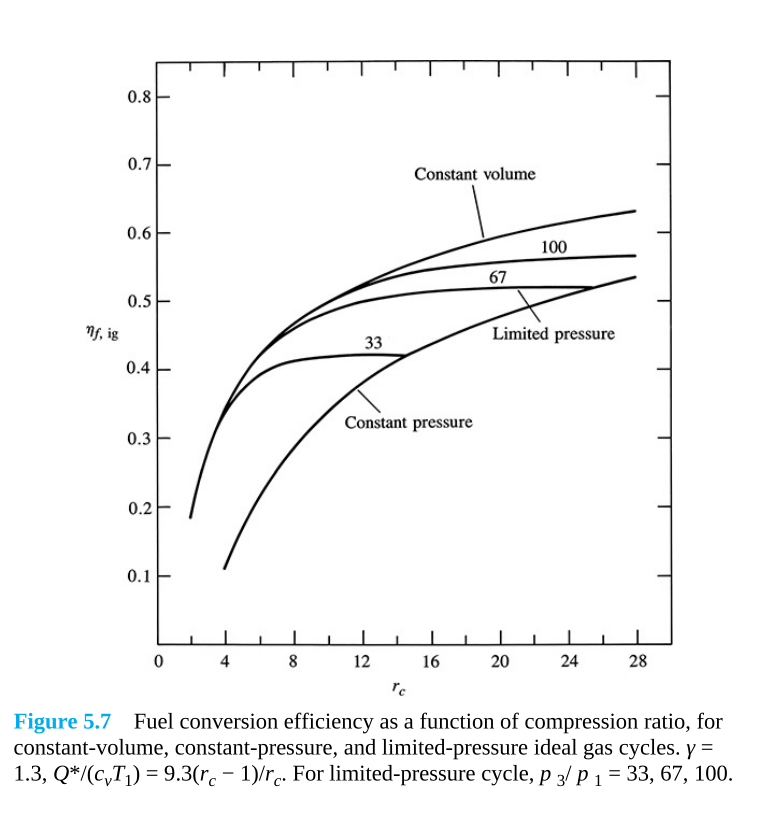
\includegraphics[width=1\textwidth]{rendimiento_conv_comb.png}
%     \caption{Comparación de rendimientos (cambiar por una imagen propia)}\label{fig:comparacion_rendimientos}
% \end{figure}
%
% El indicador que se tomará como referencia para evaluar y comparar diferentes
% geometrías es el rendimiento volumétrico ($\eta_v$), este parámetro se define
% como:
%
% \begin{equation}
%     \eta_v = \frac{m_a}{\rho_{a,i}V_d}
% \end{equation}
%
% Dónde:
% %
% \begin{description}
%     %
%     \item[$m_i$] es la masa de mezcla fresca inductada
%         %
%     \item[$\rho_{a,i}$] es la densidad del aire en el puerto de admisión
%         %
%     \item[$V_d$] es el volumen desplazado
%         %
% \end{description}
%
% El rendimiento volumétrico tiene una dependencia compleja de varios factores,
% este parámetro es el que da forma a las curvas de \emph{performance} que se
% suelen ver en literatura ya que indica la cantidad de mezcla fresca disponible
% para la combustión. 
% %
% % En caso de motores de inyección directa (tanto de CI SI)
% % NOTA: no se que quise poner aca, voy a tener que leerlo con mas de talle de
% % nuevo
%
% La combustión es estequeométrica con $a_{weibe}=5$ y $m_{weibe}=2$, el combustible utilizado
% es \emph{isooctano} con las siguientes características:
% \begin{itemize}
%     \item $y = 2.25$
%     \item $H_{vap} = 2.25 MJ/kg$
%     \item $Q_{fuel} = 44 MJ/kg_f$
% \end{itemize}
%
% La temperatura de pared se asume en 450K.

%%%%%%%%%%%%%%%%%%%%%%%%%%%%%%%%%%%%%%%%%%%%%%%%%%%%%%%%%%%%%%%%%%%%%%%%%%%%%%%

\subsection{Sistemas de intercambio de gases}
%

El eje de los tubos coincide con el eje del puerto, estos últimos hacen una
transición desde el diámetro del conducto hasta la altura de la ranura del
puerto en la cámara de combustión, en la
figura~\ref{fig:sistema_intercambio_gases} se esquematiza la geometría
mencionada.
%
En trabajos anteriores~\parencite{lopez13} se demostró que se tiene una mejor
\emph{performance} del motor si se ubican los puertos en el cuerpo central del
estator, realizando un optimización de la geometría mediante un barrido
paramétrico de las variables que determinan la forma, posición y reglaje de los
puertos, ya que es la ubicación angular de los puertos la que determina la
duración de los procesos de admisión y escape.

Para simplificar el sistema analizado, no se tuvieron en cuneta elementos
típicos de un sistema de intercambio de gases, como lo son: mariposa,
carburador, filtros de aire, convertidores catalíticos y demás.

%%%%%%%%%%%%%%%%%%%%%%%%%%%%%%%%%%%%%%%%%%%%%%%%%%%%%%%%%%%%%%%%%%%%%%%%%%%%%%%

\subsection{Simulación computacional del ciclo termodinámico del MRCVC}

El MRCVC es un motor rotativo de combustión interna encendido por chispa, en el
que gran parte de la misma ocurre a volumen constante.

ICESym utiliza modelos unidimensionales para simular el flujo en los conductos
de admisión/escape y modelos cero dimensionales o termodinámicos para la cámara
de combustión, la transferencia de calor y el modelado de la fricción.
%
Además, incluye un modelo para el solape entre cámaras~\parencite{lopez16}
entre otras modificaciones particulares al MRCVC.\@
